\documentclass{beamer}


% \usepackage{beamerthemesplit} // Activate for custom appearance
\usepackage[english]{babel}
\usepackage[T1]{fontenc}
\usepackage[utf8]{inputenc}

\usepackage{photo}
\usetheme{Berlin}
\usefonttheme{serif}
\usefonttheme[18pt]{structuresmallcapsserif}
\useinnertheme{circles}
\beamertemplatenavigationsymbolsempty
\setbeamercovered{transparent}

\usepackage{mathtools}

\usepackage{hyperref}

\usepackage{graphicx}
\graphicspath{{images/}} 
\DeclareGraphicsExtensions{.png,.jpg,.pdf}

\usepackage{multirow}
\usepackage{booktabs}
\usepackage{colortbl}
\usepackage{tabularx}
\usepackage{multirow}
\usepackage{threeparttable}
\usepackage{ragged2e}
\usepackage{makecell}


\definecolor{LITIScolor}{RGB}{1,122,175}
\setbeamercolor{structure}{fg=LITIScolor}
\usebackgroundtemplate{
\includegraphics[height=\paperheight]
{images/logoSoftBckGrd.pdf}}

\pgfdeclareimage[height=0.5cm]{logo}{TutellesLITIS}
\logo{\pgfuseimage{logo}}

\title{Knowledge Graph-based System for Technical Document Retrieval}
\subtitle{A deductive reasoning-focused exploration}
\author{Matthias Sesboüé}
\date{September 5, 2024}

\begin{document}
    \frame{
    \centering
    
\includegraphics[height = 4cm]{logoLITIS}
    
    
\includegraphics[height = 1.3cm]{TutellesLITIS}
    }
    \frame{\titlepage}
    
    \section[Table of content]{}
    \frame
    {
    \frametitle{Table of content}
    \tableofcontents
    %   \begin{columns}[t]
    % \begin{column}{5cm}
    % \tableofcontents[sections={1-4}] \end{column}
    %  \begin{column}{5cm} \tableofcontents[sections={3-4}]
    %  \end{column}
    % \end{columns}
    }
    
    % \section{Introduction}

\begin{frame}{RESPONdING thesis}
    \begin{center}
        Knowledge Graph-based System for Technical Document Retrieval\\A deductive reasoning-focused exploration
    \end{center}
    
    \begin{itemize}
        \item Research objective: Leveraging domain knowledge to enhance Information Retrieval in a technical context.
        \item CIFRE contract (financed by ANRT) between the Litis lab and the company Traceparts 
        \item Began on March 15th 2021.
    \end{itemize}
    
    \begin{center}
        From a keyword-based search to a concept-based one.
    \end{center}
    
\end{frame}

\begin{frame}{Traceparts}

    \begin{center}
        One of the world's leading CAD-content platforms for Engineering, Industrial Equipment and Machine Design. The CAD-content platform \href{http://traceparts.com/}{traceparts.com} provides access to over $1.8$ thousand supplier-certified product catalogues with 2D drawings, 3D CAD models and product datasheets.
    \end{center}

    \begin{itemize}
        \item Technical content aimed at an engineering audience from multiple industries
        \item Content available in 25 languages
        \item Users can search using :
        \begin{itemize}
            \item A full text search
            \item A list of catalogues
            \item Different classifications
        \end{itemize}
    \end{itemize}
    
    \begin{center}
        
\includegraphics[scale=0.1]{images/traceparts_logo.png}
    \end{center}
    
\end{frame}
    % Responding thesis + start date + CIFRE ANRT -> TO ENHANCE
    % Traceparts presentation -> OK

    \section{Related works}

\begin{frame}{Information Retrieval}
    
    \begin{figure} [H]
        \begin{center}
            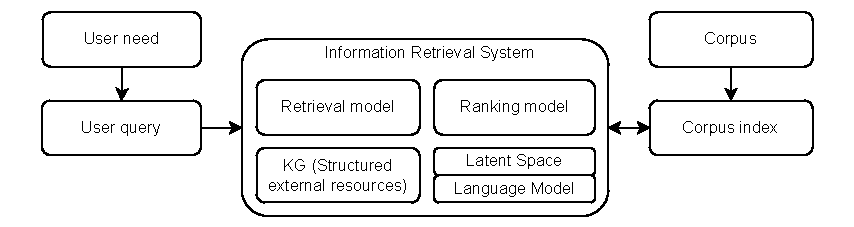
\includegraphics[scale=0.8]{images/ir-system-comps.pdf} 
            \caption{Information Retrieval System overview} 
        \end{center}
    \end{figure}

    \begin{center}
        Traditional approaches leverage statistics about the text corpus. Recent methods implement deep learning models and combines multiple approaches.
    \end{center}
    
\end{frame}

\begin{frame}{BM25}
    
    BM25 (and its many variants) is:
    \begin{itemize}
        \item based on the Term Frequencies and Inverse Document Frequencies (TF-IDF)
        \item still widely used in practice
        \item computes many statistics offline
    \end{itemize}

    \begin{center}
        Traceparts search system is largely based on a BM25 implementation.
    \end{center}
    
\end{frame}

\begin{frame}{Knowledge Graph and ontology}

    Knowledge Graph (Hogan et. al. 2021):
    \begin{center}
        \emph{a knowledge graph as a graph of data intended to accumulate and convey knowledge of the real world, whose nodes represent entities of interest and whose edges represent relations between these entities. The graph of data (aka. data graph) conforms to a graph-based data model, which may be a directed edge-labelled graph, a property graph, etc. By knowledge, we refer to something that is known.}
    \end{center}

    Ontology (Hogan et. al. 2021):
    \begin{center}
        \emph{In the context of computing, an ontology is then a concrete, formal representation of what terms mean within the scope in which they are used (e.g., a given domain).}
    \end{center}

    In our work, we consider an ontology a particular component of a Knowledge Graph
    
\end{frame}
    % SOTA IR system components -> OK
    % BM25 -> OK
    % KG definition  -> OK

    \section[KG-based system]{Knowledge Graph-Based System (KGBS)}

\begin{frame}{Knowledge Acquisition}

    \begin{figure} [H]
        \begin{center}
            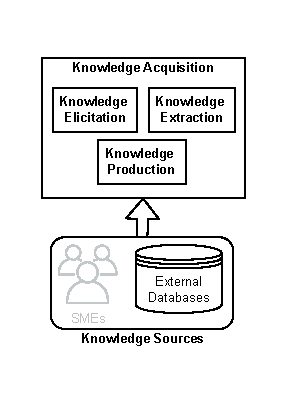
\includegraphics[scale=0.8]{images/KGBS-knowledge-acquisition.pdf} 
            \caption{KGBS: Knowledge acquisition} 
        \end{center}
    \end{figure}

\end{frame}

\begin{frame}{Knowledge modeling}

    \begin{figure} [H]
        \begin{center}
            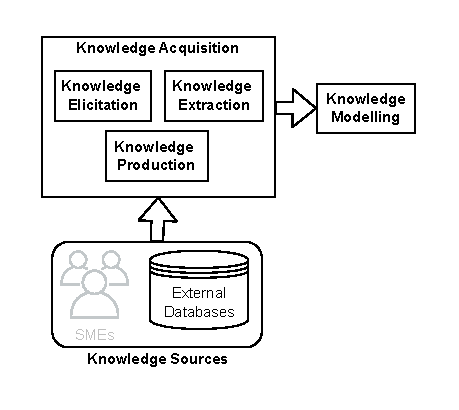
\includegraphics[scale=0.8]{images/KGBS-knowledge-modelling.pdf} 
            \caption{KGBS: Knowledge modeling} 
        \end{center}
    \end{figure}

\end{frame}

\begin{frame}{Knowledge Graph}

    \begin{figure} [H]
        \begin{center}
            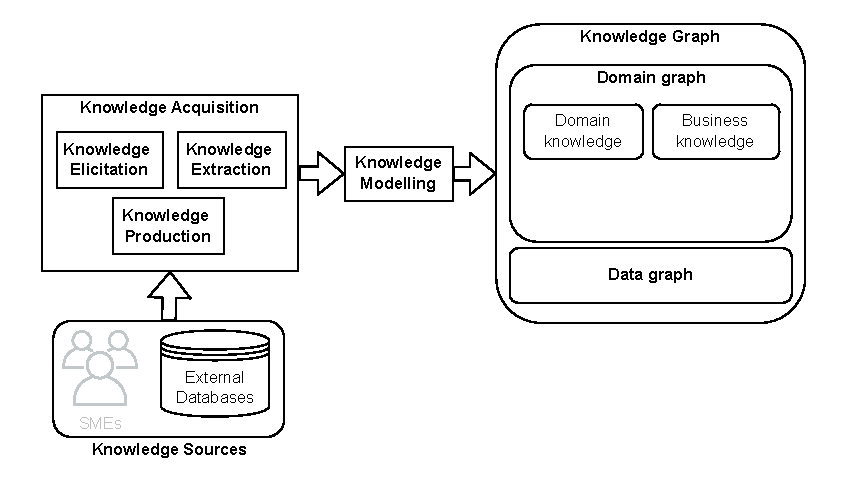
\includegraphics[scale=0.6]{images/KGBS-knowledge-modelling-kg.pdf} 
            \caption{KGBS: Knowledge Graph} 
        \end{center}
    \end{figure}

\end{frame}

\begin{frame}{Knowledge consumption}

    \begin{figure} [H]
        \begin{center}
            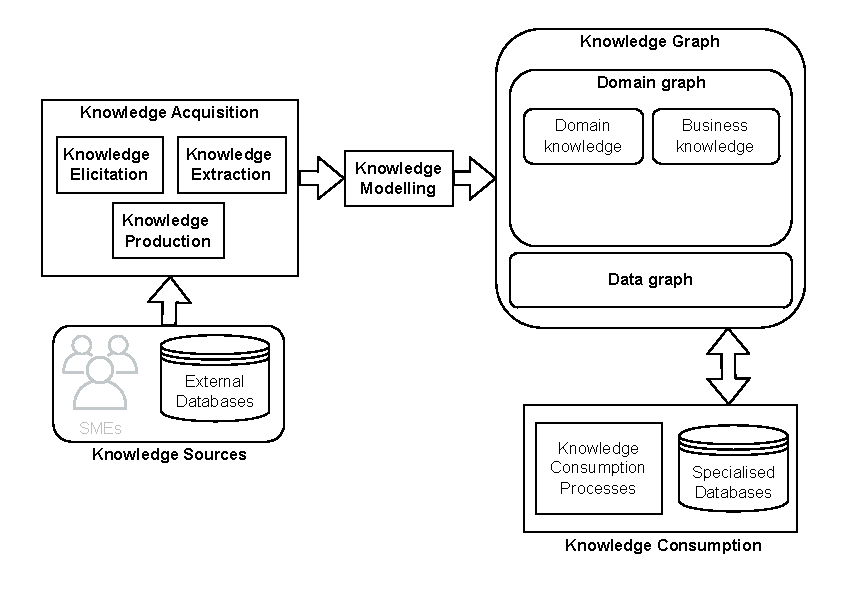
\includegraphics[scale=0.6]{images/KGBS-knowledge-consumption.pdf} 
            \caption{KGBS: knowledge consumption} 
        \end{center}
    \end{figure}

\end{frame}

\begin{frame}{Knowledge Graph-Based System architecture}

    \begin{figure} [H]
        \begin{center}
            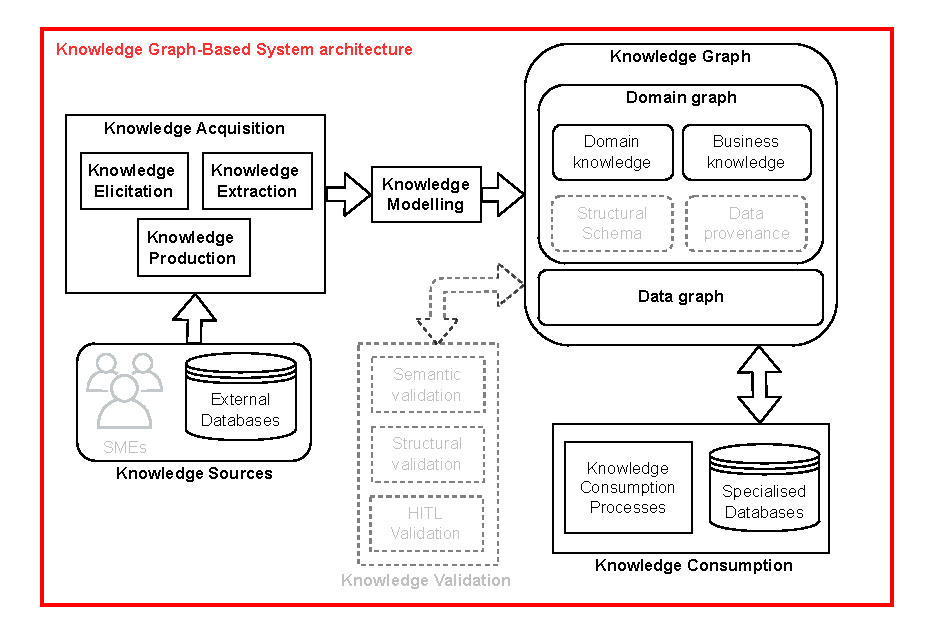
\includegraphics[scale=0.5]{images/KGBS-architecture.pdf} 
            \caption{KGBS architecture} 
        \end{center}
    \end{figure}

\end{frame}

% \begin{frame}{Knowledge Graph vs Ontology}

%     \begin{figure} [H]
%         \begin{center}
%             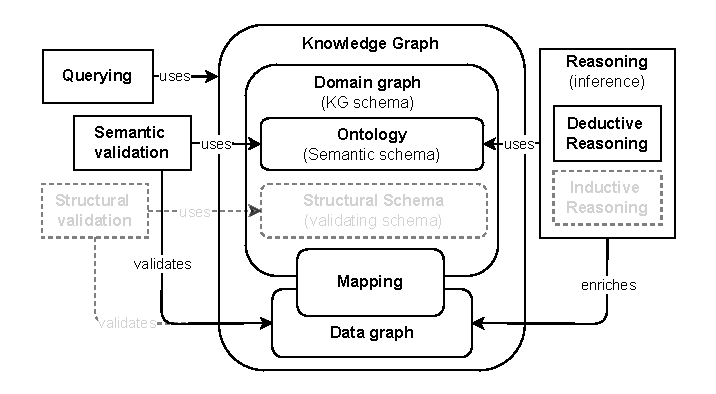
\includegraphics[scale=0.8]{images/kg-def-simple.pdf} 
%             \caption{Knowledge Graph definition} 
%         \end{center}
%     \end{figure}

% \end{frame}

\begin{frame}{Ontology Learning Applied Framework (OLAF)}

    \begin{figure} [H]
        \begin{center}
            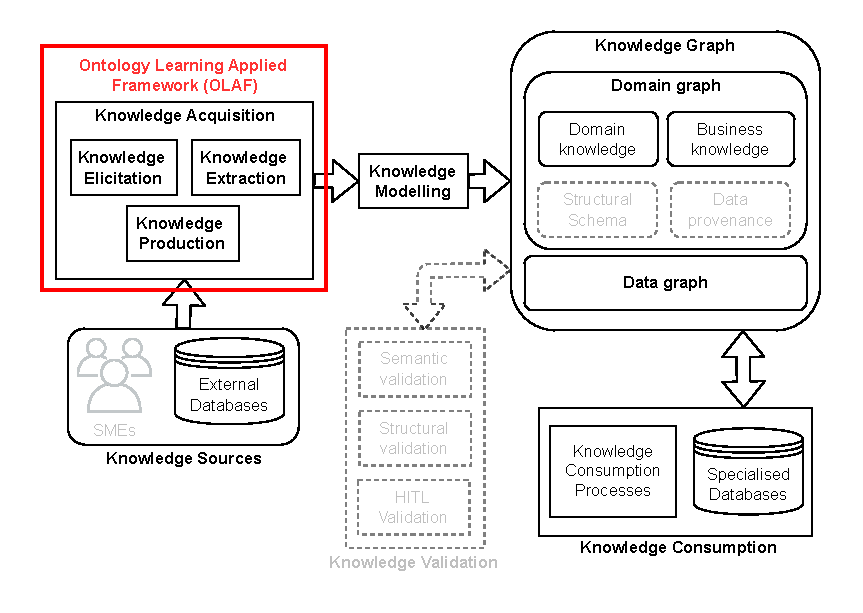
\includegraphics[scale=0.5]{images/KGBS-knowledge-acquisition-OLAF.pdf} 
            \caption{KGBS architecture: OLAF} 
        \end{center}
    \end{figure}

\end{frame}

\begin{frame}{Information Retrieval ontology}

    \begin{figure} [H]
        \begin{center}
            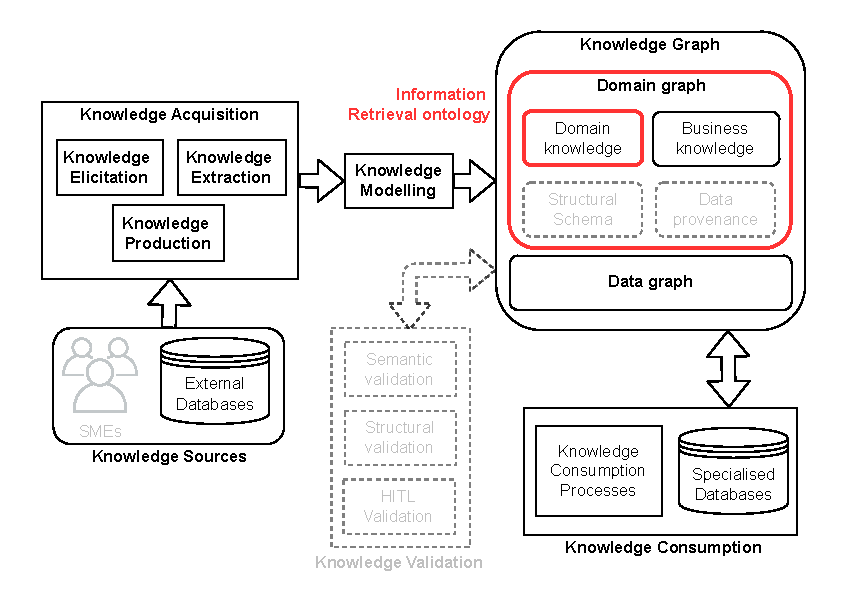
\includegraphics[scale=0.5]{images/KGBS-knowledge-modelling-kg-IR-onto.pdf} 
            \caption{KGBS architecture: IR ontology} 
        \end{center}
    \end{figure}

\end{frame}

\begin{frame}{Industrial experiments}

    \begin{figure} [H]
        \begin{center}
            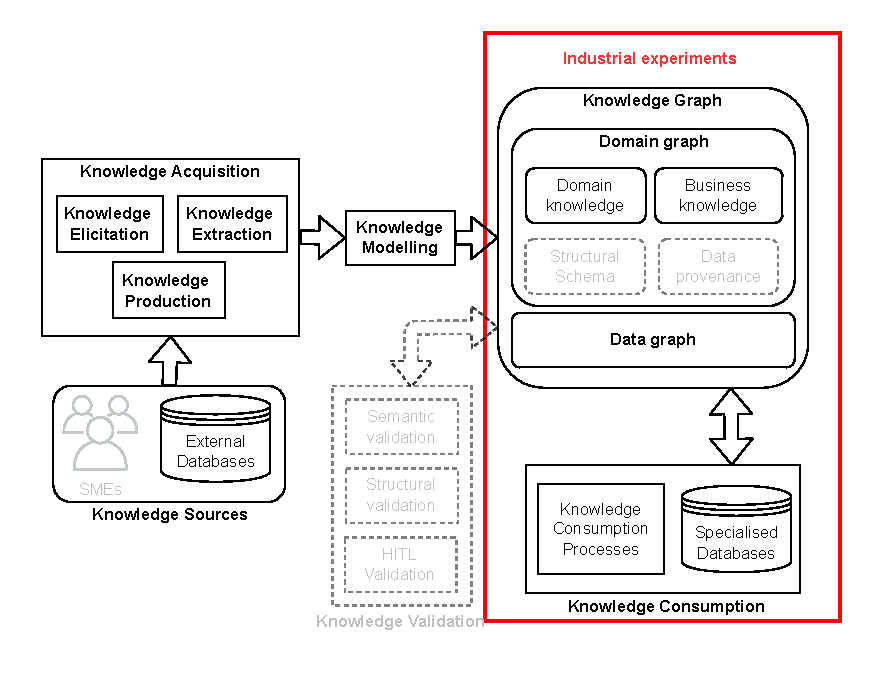
\includegraphics[scale=0.5]{images/KGBS-knowledge-consumption-industrial-exp.pdf} 
            \caption{KGBS architecture: Industrial experiments} 
        \end{center}
    \end{figure}

\end{frame}

\begin{frame}{In this presentation}

    \begin{figure} [H]
        \begin{center}
            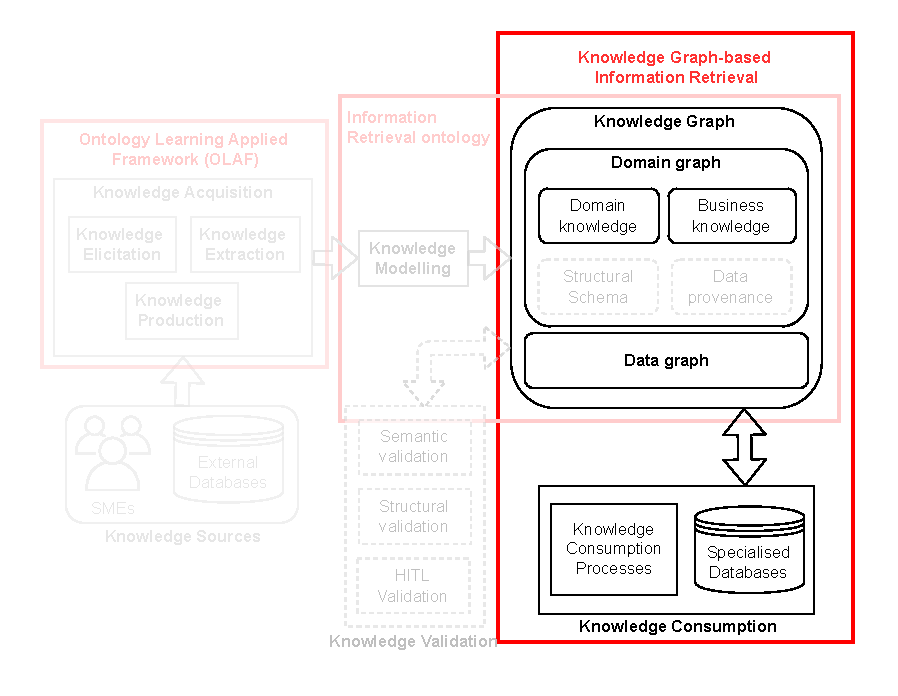
\includegraphics[scale=0.5]{images/KGBS-architecture-focus-TP-expe.pdf} 
            \caption{This presentation KGBS architecture components focus} 
        \end{center}
    \end{figure}

\end{frame}
    % iteratively introduce each components  -> OK
    % end up with red squares on each parts to introduce our contributions  -> OK

    \section{Application context}

\begin{frame}{Corpus}
    
    \begin{itemize}
        \item Over $1.1$ million document families
        \item Over $127.8$ millions individual documents
        \item $25$ languages
        \item Documents' texts contain average $50$ characters and $7$ words
        \item Over $210$ thousand tags, amongst which:
        \begin{itemize}
            \item Over $2.5$ thousand suppliers and manufacturers
            \item Over $1.9$ thousand catalogues
            \item Over $208$ thousand categories
        \end{itemize}
    \end{itemize}

    Some text content examples are:
    \begin{itemize}
        \item \emph{DIN 912}
        \item \emph{The P01 to P08 pumps are designed to pump lubricating fluids (oil, diesel oil, etc.). Their flow rate is from 1 to 24 L / min; maximum working pressure 10 bar.} 
    \end{itemize}

\end{frame}

\begin{frame}{User searches}
    
    User text searches:
    \begin{itemize}
        \item are composed of domain-specific keywords, notations, identifiers, and
        acronyms.
        \item contain on average 13 characters separated into 2 words.
        \item can come in any languages
    \end{itemize}

    Some common search examples are:
    \begin{center}
        \emph{motor}, \emph{din 912}, and \emph{ball valve}.
    \end{center}
    
\end{frame}

\begin{frame}{Traceparts search system challenges}
    
    Traceparts search challenges come from:
    \begin{itemize}
        \item Short multilingual texts
        \item Technical texts with many synonyms, acronyms, homonyms, and notations
        \item A large and heterogeneous corpus
        \item Multiple engineering domains coverage
        \item High recall but low precision
    \end{itemize}

\end{frame}

% \begin{frame}{Traceparts search system}
    
%     \begin{figure} [H]
%         \begin{center}
%             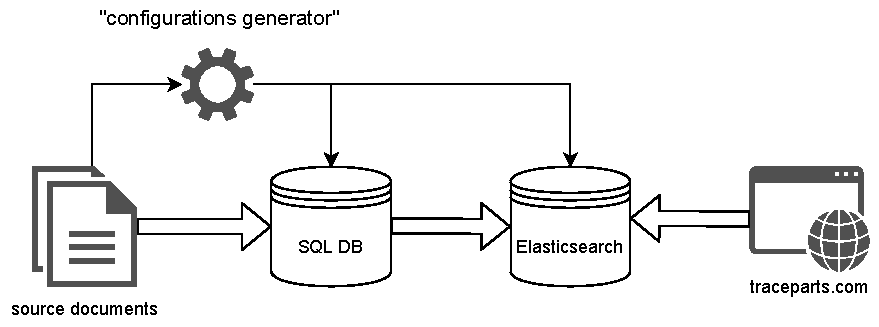
\includegraphics[scale=0.7]{images/tp_system.pdf} 
%             \caption{Traceparts current system} 
%         \end{center}
%     \end{figure}

%     \begin{center}
%         Parts configurations are generated with their text content to be searchable.    
%     \end{center}
    
% \end{frame}
    % Description des utilisateurs
    % Searches descriptions (+ examples) -> OK
    % Description des données (+ examples) -> OK
    % Description des possibilité de recherche (text, categories, catalogues)
    % TP search system limitations (short texts, mulitlingual text, technical text, acronyms, notations, homonyms, synonyms ...) -> OK
    % TP search system (+ diagram) -> OK
    
    \section{KG-based Information Retrieval system}

\begin{frame}{Experiments objective}

    \begin{center}
        From a text-based to a concept-based search.
    \end{center}

    \begin{figure} [H]
        \begin{center}
            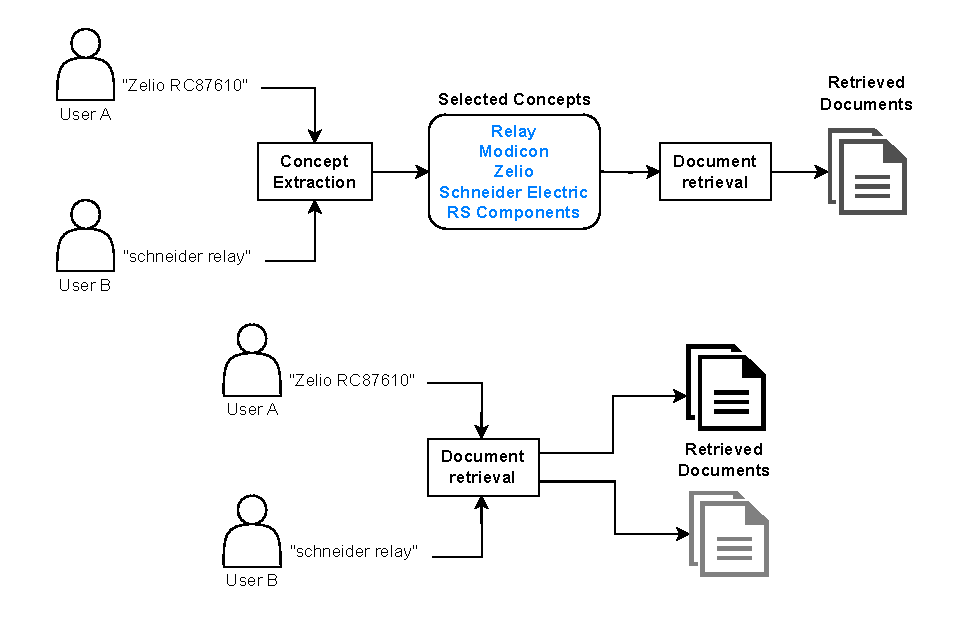
\includegraphics[scale=0.6]{images/text-vs-concept-based-search.pdf} 
            \caption{Text-based vs concept-based search.} 
        \end{center}
    \end{figure}

\end{frame}

\begin{frame}{Evaluation metrics}

    \begin{itemize}
        \item Mean Average Precision at k (MAP@k): 
        \begin{itemize}
            \item A sliding (or growing) precision window, averaged over a set of query examples.
            \item Ranges from $0$ to $1$ ($1$ is the best value).
            \item Gives information about the amount and positions of positive results in the k first ones.
        \end{itemize}
        \item Binary Mean at k (BM@k):
        \begin{itemize}
            \item Binary average over a set of query examples.
            \item Ranges from $0$ to $1$ ($1$ is the best value).
            \item Provides information about the amount of queries with a positive result in the k first ones.
            \item Does not give any detail on the positive result position.
        \end{itemize}
    \end{itemize}

\end{frame}
    % objective: text-based vs concept-based system -> OK
    % introduce experiments systems with a growing diagram -> TODO
    % Evaluation metrics + results for TP system? -> ADD TP SYSTEM VALUES

    \section{First approach for KG-based IR system}

\begin{frame}{Experiments objective}

    \begin{center}
        From a text-based to a concept-based search.
    \end{center}

    \begin{figure} [H]
        \begin{center}
            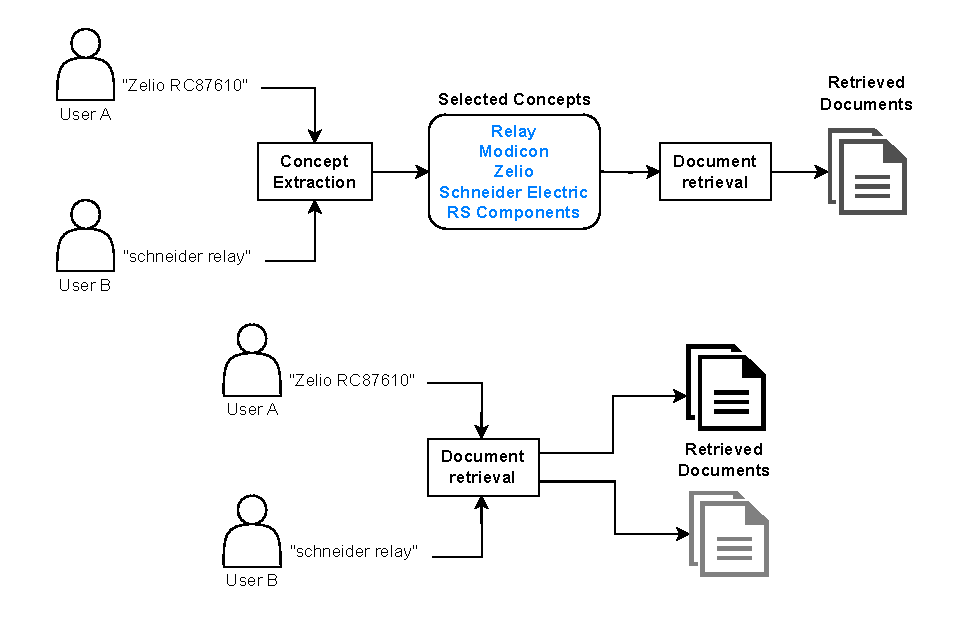
\includegraphics[scale=0.6]{images/text-vs-concept-based-search.pdf} 
            \caption{Text-based vs concept-based search.} 
        \end{center}
    \end{figure}

\end{frame}

\begin{frame}{Experiments protocol}

    \begin{figure} [H]
        \begin{center}
            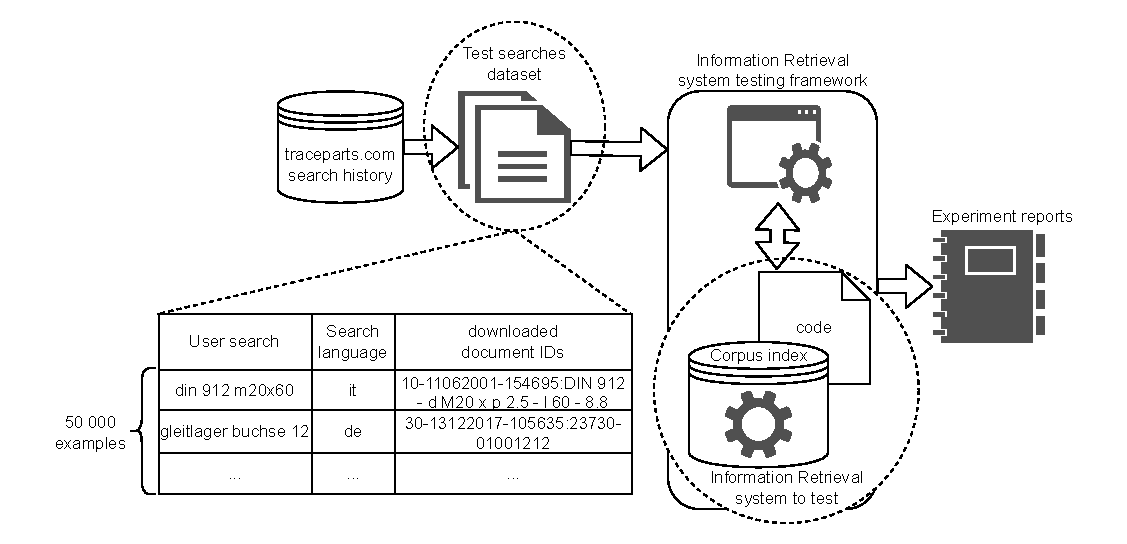
\includegraphics[scale=0.6]{images/tp-search-expe-setting.pdf} 
            \caption{Experiments Protocol.} 
        \end{center}
    \end{figure}

\end{frame}

\begin{frame}{Information Retrieval systems}

    6 distinct systems built iteratively:
    \begin{itemize}
        \item Text-based system (baseline)
        \item Concept-based system
        \item Knowledge Graph-based system
        \item Text-based system with implicit knowledge
        \item Concept-based system with implicit knowledge
        \item Knowledge Graph-based system with implicit knowledge
    \end{itemize}

    Implementation:
    \begin{itemize}
        \item User search concept matching problem as an information retrieval task.
        \item Leverage user search history as implicit knowledge.
        \item Query concept enrichment as a graph traversal task.
    \end{itemize}

\end{frame}

\begin{frame}{Information Retrieval systems}

    \begin{figure} [H]
        \begin{center}
            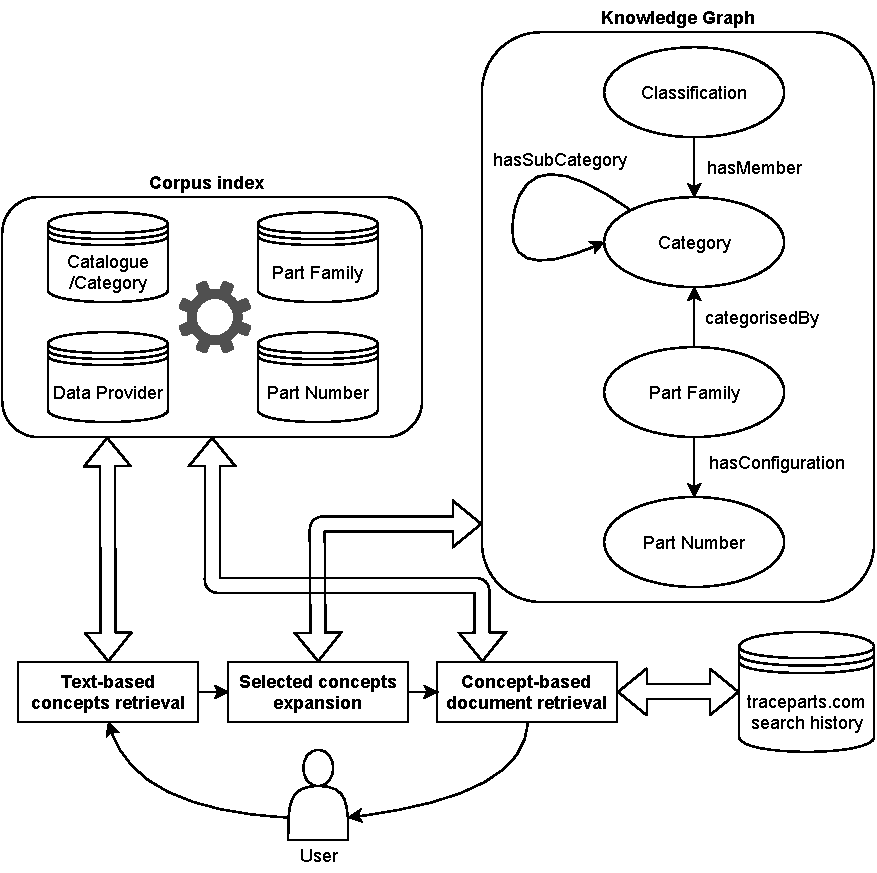
\includegraphics[scale=0.45]{images/kg-based-ir-system-with-search-hist.pdf} 
            \caption{Knowledge Graph-based system with implicit knowledge.} 
        \end{center}
    \end{figure}

\end{frame}


\begin{frame}{Results}

    % \begin{table}[htbp]
    %     \small
    %     \centering
    %     \begin{tabular}{c|cc|cc|cc|}
    %         \toprule
    %         \multicolumn{1}{l}{}               & \multicolumn{3}{c}{\textbf{Text-based system (baseline)}}                                & \multicolumn{3}{c}{\textbf{Concept-based system}}                                         & \multicolumn{3}{c}{\textbf{\begin{tabular}[c]{@{}c@{}}KG-based system\\with search history\end{tabular}}}                                             \\ \cmidrule(lr){2-10} %\cmidrule(lr){2-4}\cmidrule(lr){5-7}\cmidrule(lr){8-10}
    %         \multicolumn{1}{c|}{\textbf{@k $\downarrow$}}    & \multicolumn{1}{c}{\textbf{MAP@k}}  & \textbf{BM@k} & \multicolumn{1}{|c}{\textbf{MAP@k}} & BM@k  & \multicolumn{1}{|c}{\textbf{MAP@k}} & \textbf{BM@k} \\ \cmidrule(lr){2-10}
    %         \multicolumn{1}{c|}{\textbf{@5}}   & \multicolumn{1}{c}{0.061}          & 0.114         & \multicolumn{1}{|c}{0.152} & 0.243 & \multicolumn{1}{|c}{0.115}          & \textbf{0.291}        \\ 
    %         \multicolumn{1}{c|}{\textbf{@25}}  & \multicolumn{1}{c}{0.064}          & 0.148         & \multicolumn{1}{|c}{0.159} & 0.334 & \multicolumn{1}{|c}{0.122}          & \textbf{0.471}         \\ 
    %         \multicolumn{1}{c|}{\textbf{@50}}  & \multicolumn{1}{c}{0.064}          & 0.157         & \multicolumn{1}{|c}{0.160} & 0.371 & \multicolumn{1}{|c}{0.123}          & \textbf{0.552}         \\ 
    %         \multicolumn{1}{c|}{\textbf{@100}} & \multicolumn{1}{c}{0.064}          & 0.161         & \multicolumn{1}{|c}{0.161} & 0.403 & \multicolumn{1}{|c}{0.123}          & \textbf{0.624}         \\ 
    %         \multicolumn{1}{c|}{\textbf{@350}} & \multicolumn{1}{c}{0.064}          & 0.164         & \multicolumn{1}{|c}{0.161} & 0.429 & \multicolumn{1}{|c}{0.124}          & \textbf{0.715}         \\ \bottomrule
    %     \end{tabular}
    %     \caption{
    %         Comparing text, concept, and KG-based systems on the Part Family (PF) corpus for different k values.
    %     }\label{tab:comp-text-concept-kg}
    % \end{table} 

\end{frame}

\begin{frame}{Results}

    % \begin{table}[htbp]
    %     \centering
    %     \begin{tabular}{ccc}
    %         \toprule
    %         {} &  \textbf{No results}  &  \textbf{\begin{tabular}[c]{@{}c@{}}Less than 400\\ results (non empty)\end{tabular}} \\
    %         \midrule
    %         \textbf{Text-based system (baseline)}              &     64.48\% &              35.44\% \\
    %         \textbf{Concept-based system}                      &     11.43\% &              \textbf{88.36\%} \\
    %         \textbf{KG-based system with search history}      &     \textbf{8.10\%} &       51.59\% \\
    %         \bottomrule
    %     \end{tabular}
    %     \caption{
    %         Comparing all search systems results set on the Part Family (PF) corpus.
    %     }\label{tab:comp-all-sys-res-list}
    % \end{table}

\end{frame}
    % Experiment protocol -> OK
    % + implementation details -> OK

    % \section{Results}

% Iteratively introduce the main systems (Text -> Concept -> KG + implicit knowledge)
% Present the system in a small snippet ?

\begin{frame}{Qualitative results}

    % \begin{table}[htbp]
    %     \begin{center}
    %     \small
    %     \begin{tabular}{c|cc|cc|cc|}
    %         \toprule
    %         \multicolumn{1}{l}{}               & \multicolumn{2}{c}{\textbf{\begin{tabular}[c]{@{}c@{}}Text-based\\ system (baseline)\end{tabular}}}  & \multicolumn{2}{c}{\textbf{\begin{tabular}[c]{@{}c@{}}Concept-based\\ system\end{tabular}}} & \multicolumn{2}{c}{\textbf{\begin{tabular}[c]{@{}c@{}}KG-based system\\with search history\end{tabular}}} \\ \cmidrule(lr){2-7} %\cmidrule(lr){2-4}\cmidrule(lr){5-7}\cmidrule(lr){8-10}
    %         \multicolumn{1}{c|}{\textbf{@k $\downarrow$}}    & \multicolumn{1}{c}{\textbf{MAP@k}}  & \textbf{BM@k} & \multicolumn{1}{|c}{\textbf{MAP@k}} & \textbf{BM@k}  & \multicolumn{1}{|c}{\textbf{MAP@k}} & \textbf{BM@k} \\ \cmidrule(lr){2-7}
    %         \multicolumn{1}{c|}{\textbf{@5}}   & \multicolumn{1}{c}{0.061}          & 0.114         & \multicolumn{1}{|c}{0.152} & 0.243 & \multicolumn{1}{|c}{0.115}          & \textbf{0.291}        \\ 
    %         \multicolumn{1}{c|}{\textbf{@25}}  & \multicolumn{1}{c}{0.064}          & 0.148         & \multicolumn{1}{|c}{0.159} & 0.334 & \multicolumn{1}{|c}{0.122}          & \textbf{0.471}         \\ 
    %         \multicolumn{1}{c|}{\textbf{@50}}  & \multicolumn{1}{c}{0.064}          & 0.157         & \multicolumn{1}{|c}{0.160} & 0.371 & \multicolumn{1}{|c}{0.123}          & \textbf{0.552}         \\ 
    %         \multicolumn{1}{c|}{\textbf{@100}} & \multicolumn{1}{c}{0.064}          & 0.161         & \multicolumn{1}{|c}{0.161} & 0.403 & \multicolumn{1}{|c}{0.123}          & \textbf{0.624}         \\ 
    %         \multicolumn{1}{c|}{\textbf{@350}} & \multicolumn{1}{c}{0.064}          & 0.164         & \multicolumn{1}{|c}{0.161} & 0.429 & \multicolumn{1}{|c}{0.124}          & \textbf{0.715}         \\ \bottomrule
    %     \end{tabular}
    %     \caption{
    %         Comparing text, concept, and KG-based systems for different k values.
    %     }\label{tab:comp-text-concept-kg}
    % \end{center}
    % \end{table} 

\end{frame}

\begin{frame}{Quantitative results}

    % \begin{table}[htbp]
    %     \begin{center}
    %     \small
    %     \begin{tabular}{ccc}
    %         \toprule
    %         {} &  \textbf{No results}  &  \textbf{\begin{tabular}[c]{@{}c@{}}Less than 400\\ results (non empty)\end{tabular}} \\
    %         \midrule
    %         \textbf{\begin{tabular}[c]{@{}c@{}}Text-based\\ system (baseline)\end{tabular}}              &     64.48\% &              35.44\% \\
    %         \textbf{\begin{tabular}[c]{@{}c@{}}Concept-based\\ system\end{tabular}}                      &     11.43\% &              \textbf{88.36\%} \\
    %         \textbf{\begin{tabular}[c]{@{}c@{}}KG-based system\\with search history\end{tabular}}      &     \textbf{8.10\%} &       51.59\% \\
    %         \bottomrule
    %     \end{tabular}
    %     \caption{
    %         Comparing all search systems results set corpus.
    %     }\label{tab:comp-all-sys-res-list}
    % \end{center}
    % \end{table}

\end{frame}
    % Diagram of the TP text-based system with the baseline results -> OK
    % With a growing table (and a recall of the systems diagrams?) introduce concept-based and KG-based system results -> OK
    
    \section{Second approach: online OWL reasoning-based system}

\begin{frame}{Online OWL reasoning-based approach}

    A second approach focusing on OWL.
    
    \begin{itemize}
        \item An Information Retrieval ontology.
        \item Push knowledge closer to the data.
        \item Model domain knowledge as sets of taxonomies. 
    \end{itemize}

\end{frame}

\begin{frame}{Knowledge modelling}

    \begin{figure} [H]
        \begin{center}
            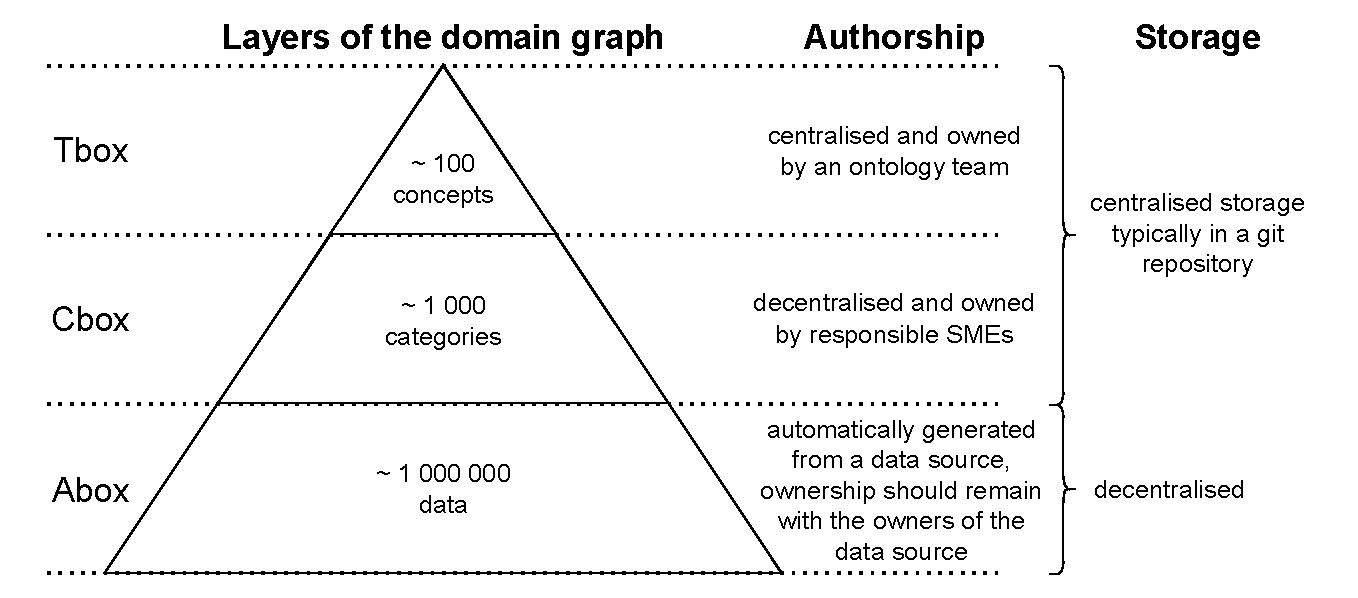
\includegraphics[scale=0.5]{images/TboxAboxCboxLayers.pdf} 
            \caption{"C-box" knowledge modelling approach} 
        \end{center}
    \end{figure}

\end{frame}

\begin{frame}{Information Retrieval Ontology}

    Competency questions:
    \begin{itemize}
        \item CQ1 What are the categories in the user search?
        \item CQ2 What are the documents relevant to a search?
        \item CQ3 What categories are enabled to refine the search?
    \end{itemize}

    7 classes:
    \begin{itemize}
        \item \emph{Candidate Document} subclass of \emph{Document} 
        \item \emph{Selected Category} and \emph{Enabled Category} subclasses of \emph{Category}
        \item \emph{Search Context} subclass of \emph{Search}
    \end{itemize}

    6 Object properties:
    \begin{itemize}
        \item \emph{categorises} inverse of \emph{categorised By}
        \item \emph{has Search Category} subproperty of \emph{enables Category}
        \item \emph{has Direct Subcategory} subproperty of \emph{has Subcategory}
    \end{itemize}

\end{frame}

\begin{frame}{Knowledge Graph}

    \begin{figure} [H]
        \begin{center}
            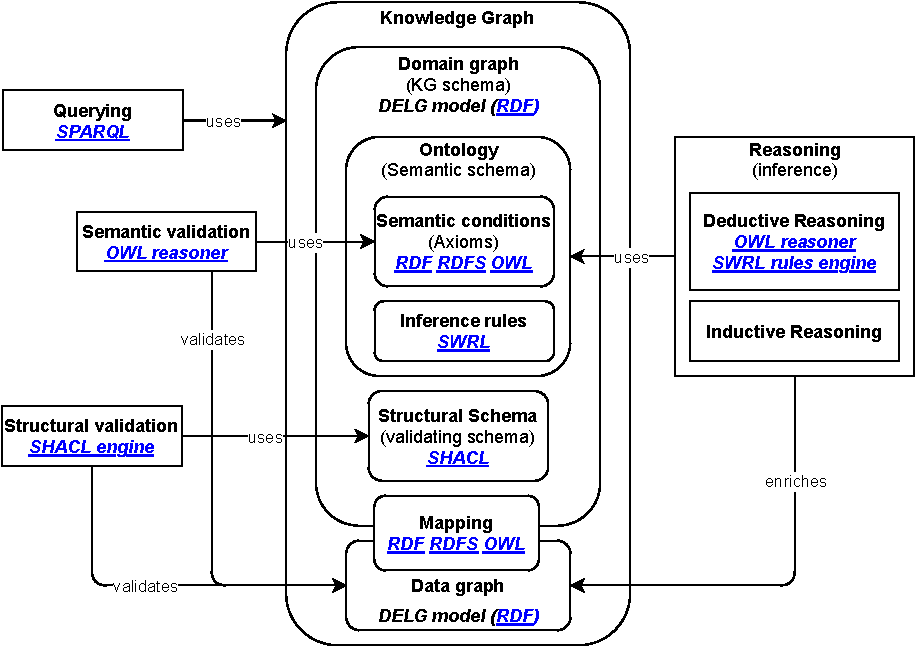
\includegraphics[scale=0.6]{images/manuscript-chap1-summary-technos.pdf} 
            \caption{Knowledge Graph definition} 
        \end{center}
    \end{figure}
    % Introduce the figure with technologies to introduce the pizza ontology demo
    % Lighten parts not used

\end{frame}

\begin{frame}{Pizza ontology Knowledge Graph}

    \begin{figure} [H]
        \begin{center}
            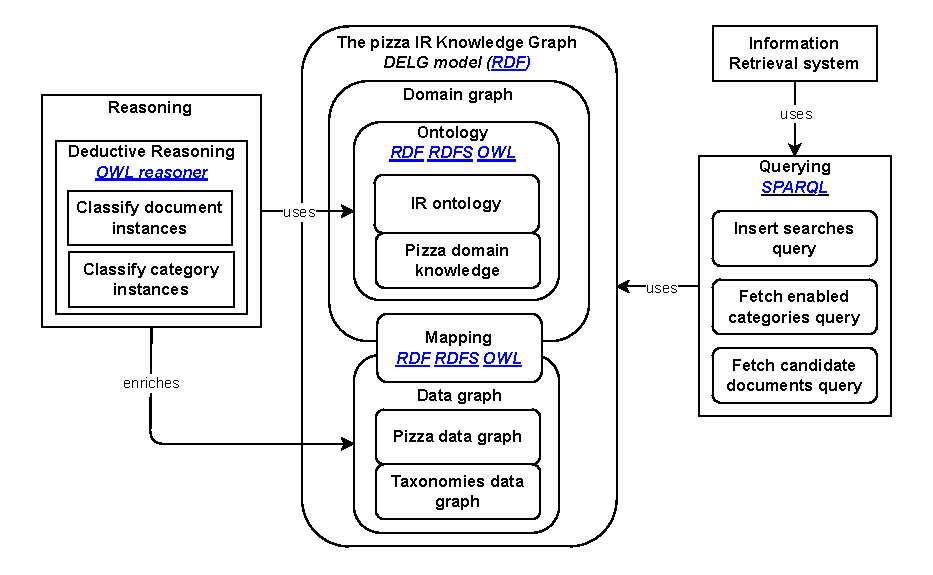
\includegraphics[scale=0.7]{images/pizza-demo-kg.pdf} 
            \caption{Pizza ontology Knowledge Graph} 
        \end{center}
    \end{figure}
\end{frame}


\begin{frame}{OWL reasoning-based Information Retrieval}

    \begin{figure} [H]
        \begin{center}
            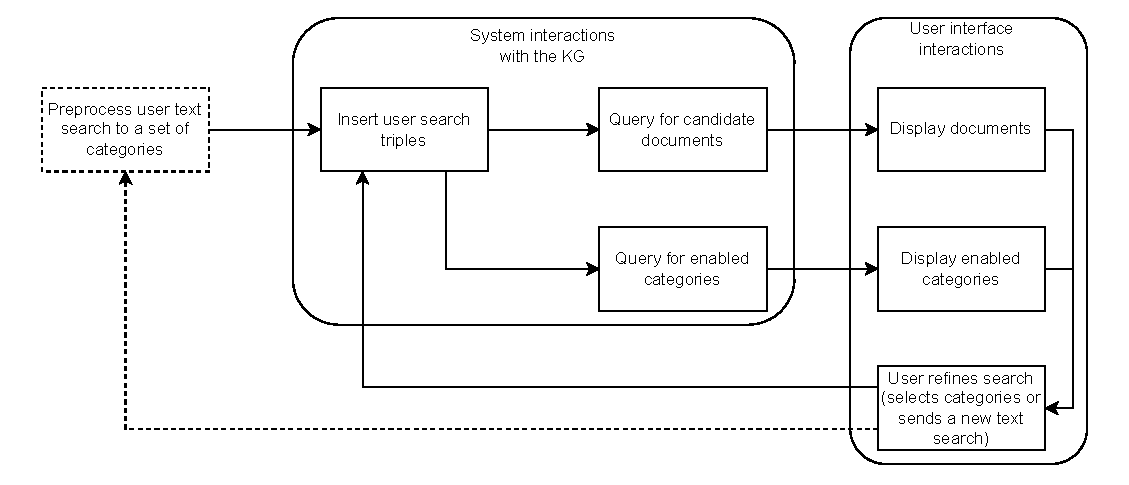
\includegraphics[scale=0.5]{images/ir-onto-search-process.pdf} 
            \caption{OWL reasoning-based Information Retrieval process.} 
        \end{center}
    \end{figure}
\end{frame}

    % Focus on knowledge modeling for IR, Our second exploratory approach (we try to push as much knowledge as possible down to the KG), Novelty of this approach : OWL reasoning mostly used offline, we propose to use it at runtime (in IR) (Stream reasoning) -> OK
    % Knowledge modelling approach (C-box diagram) -> OK
    % Our proposed ontology: IR ontology -> OK
    % Pizza ontology as an example because of time constraints, Pizza onto is composed of pizzas, ingredients, pizza bases etc. -> TO COMPLETE
    % Align with the KG definition -> OK
    % Process diagram ? + example of searches and results -> TODO

    \section[Conclusion]{Conclusion and future works}

\begin{frame}{Conclusion}

    We have:
    \begin{itemize}
        \item Explored a Knowledge Graph-Based System (KGBS) architecture
        \item Detailed each KGBS containers and activities
        \item Explored a real-world use case moving from a text-based to a KG-based Information Retrieval (IR) System.
        \item Introduce and compared $3$ IR systems:
        \begin{itemize}
            \item A text-based IR system
            \item A concept-based IR system
            \item A KG-based IR system
        \end{itemize}
    \end{itemize}

     \begin{center}
        KG-based systems for IR on a multi corpus of technical documents show promising results overcoming the text-based approaches limitations.   
     \end{center}

\end{frame}

\begin{frame}{Future works}

    \begin{itemize}
        \item KGBS architecture:
        \begin{itemize}
            \item Implement an end-to-end Knowledge Graph-Based System architecture use case.
            \item Further explore the modularity of the architecture
        \end{itemize}
        \begin{itemize}
            \item 
        \end{itemize}
        \item Knowledge Graph-based Information Retrieval system:
        \begin{itemize}
            \item Expand the Knowledge Graph
            \item Enhance the concept matching task
            \item Expand the approach to other domains
        \end{itemize}
    \end{itemize}

\end{frame}

\begin{frame}{Perspectives: Knowledge Graph}

    \begin{figure} [H]
        \begin{center}
            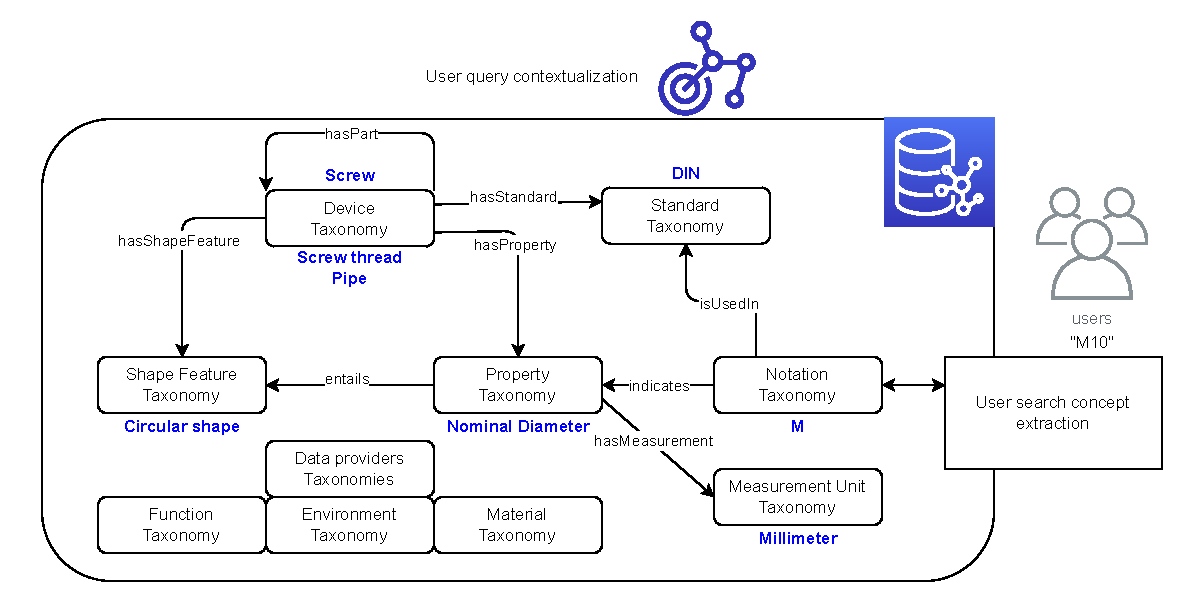
\includegraphics[scale=0.5]{images/semantic_search_example.pdf} 
            \caption{Extended semantic search example.} 
        \end{center}
    \end{figure}

\end{frame}

\begin{frame}{Contributions}

    \begin{center}
        A top-down approach from a system perspective down to solution implementations.
    \end{center}

    Contributions:
    \begin{itemize}
        \item A unifying definition of Knowledge Graph
        \item An architecture for Knowledge Graph-Based Systems
        \item A framework for Ontology Learning
        \item An OWL Information Retrieval ontology
        \item A study of a text-based compared to a Knowledge Graph-based Information Retrieval system
    \end{itemize}
    
\end{frame}

\begin{frame}{Scientific productions}

    Peer-reviewed international conference papers:
    \begin{itemize}
        \item An operational architecture for knowledge graph-based systems. Proceedings of the 26th International Conference KES2022.
        \item (with Marion Schaeffer) Olaf: An ontology learning applied framework. Proceedings of the 27th International Conference KES2023.
    \end{itemize}

    Open-source software library (with Marion Schaeffer):
    \begin{itemize}
        \item Ontology Learning Applied Framework Python library implementation:\\\href{https://wikit-ai.github.io/olaf/}{https://wikit-ai.github.io/olaf/}
    \end{itemize}

\end{frame}
    % Contributions -> OK
    % We implemented only portions of our KGBS -> OK
    % We did not touch on OLAF there but it is continuously developped by Marion -> OK
    % Expand the KG for Traceparts (+ diagram dream onto-based system) -> OK
    % Publications -> OK
    
    \begin{frame}{Thank you!}
    
    \begin{center}
    Thank you for your attention, any questions?
    \end{center}
    
\end{frame}

    % \begin{frame}{Knowledge Graph Based system}
    
    % \begin{figure} [H]
    %     \begin{center}
    %         \includegraphics[scale=0.6]{images/.pdf} 
    %         \caption{Experiments Protocol.} 
    %     \end{center}
    % \end{figure}

\end{frame}

\begin{frame}{Knowledge Graph Based system}
    
    % \begin{figure} [H]
    %     \begin{center}
    %         \includegraphics[scale=0.6]{images/.pdf} 
    %         \caption{Experiments Protocol.} 
    %     \end{center}
    % \end{figure}

\end{frame}

\begin{frame}{Information Retrieval ontology}
    
    \begin{Verbatim}
        :SelectedCategory rdf:type owl:Class ;
                rdfs:subClassOf :Category ,
                                [ rdf:type owl:Restriction ;
                                    owl:onProperty :categorises ;
                                    owl:allValuesFrom :CandidateDocument
                                ] ,
                                [ rdf:type owl:Restriction ;
                                    owl:onProperty :enablesCategory ;
                                    owl:allValuesFrom :EnabledCategory
                                ] ,
                                [ rdf:type owl:Restriction ;
                                    owl:onProperty :hasSubcategory ;
                                    owl:allValuesFrom :SelectedCategory
                                ] .
    
        :SearchContext rdf:type owl:Class ;
                    rdfs:subClassOf :Search ,
                                    [ rdf:type owl:Restriction ;
                                        owl:onProperty :hasSearchCategory ;
                                        owl:allValuesFrom :SelectedCategory
                                    ] .
    \end{Verbatim}

\end{frame}

\end{document}